

\section{Water Sampling} \label{sampling}

For the summer of 2017 a total of 29 inland lakes were sampled.  Prior to sampling, permission of riparian owner was obtained for most lakes which did not have public access. Sample surveying began on the month of June 2017 until October 2017. Each month every lake one was sampled once. Sampling locations were chosen from known list of lakes reported with HABs and existing collaborative partners. In addition, we also chose lakes that are reasonably close to I-75 expressway for the ease of transportation. See table \ref{table:Surveyed Lakes} for the list of sampled lake observed in our analysis and figure \ref{overview} for a map of our lake sites.

Water samples were collected by wading in toward the center of the lake until water height reached waist height. All water grab samples were taken roughly one foot below water surface.

Few of the lakes had public access areas for our sampling site. A total of 4 team of field surveyors sampled each with designated lakes. At each lake a hand-held multi-meter was used to measure pH, conductivity ($\mu$S/cm), dissolved oxygen (mg/L) and temperature ($^\circ$C). Phycocyanin and chlorophyll fluorescence were also measured using an Amiscience portable  with the optical excitation of 470nm and 590nm and the emission is read at 685nm, which is measured in relative fluorescence units (RFU). Each fluorometer for each lakey surveyor was calibrated against rhodamine WT dye as a secondary calibration standard, which ensure the data is relative to all other fluorometer. A portable HACH turbidity meter was used to measure turbidity in nephelometric turbidity unit (NTU). Formazin standards are used to calibrate the turbidity meter.



In July 2017 a constructed sampler float was installed at each lake. The sampler was constructed by the Dr. Raffel's team, which consisted with 3 plexi-glass plates and placed at each sampling location for the purpose of collecting zebra and quagga mussels (see figure \ref{samplerr}). The stack of three square plexiglass sheets are about 15,20, and 25cm in diameter which gives them a total surface area of 0.23 m$^2$ per sampler. Majority of sampler were installed on the riparian owner's dock or as a float. With the permission of riparian owners, the float is left in place for the  HOBO Pendant\texttrademark temperature and light logger were installed on floats at each lake site. Data was logged from July to October. In October, we collected the samplers and scraped all mussels into a glass mason jar for analysis of biomass. In addition, also installed a slotted PVC pipe which contains a Solid Phase Adsorbtion Toxin Tracking bag (SPATTS), a beta test of a new method of monitoring toxins. See appendix \ref{spattss} for more details.


Water sampling kits were prepared by storing pre-labeled water vessels stored in zip-lock bags for each lake. This was to prevent cross-contamination between different lake water samples during sampling transport and storage. Each sampling kit contained 60mL polyetheylene terephthalate (PETG) vials for microcystin analysis, 100mL sterile IDEXX\texttrademark bottles for QPCR analysis, 50mL polypropylene centrifuge vials and 250 mL HPDE Nalgene bottles for nutrient analysis. Each kit also provided alkaline lugols iodine solution for preserving cyanobacteria samples for identification and 6M \ch{H2SO4} for acid preservation of nutrient samples.



\begin{table}
\caption{List of surveyed Lakes with geographic location of sampling point}
\label{table:Surveyed Lakes}
\begin{center}
\scalebox{0.86}{
\begin{tabular}{|l|l|l|r|r|l|}
\multicolumn{1}{|c|}{Name of Lake} & \multicolumn{1}{c|}{Shorten Code} & \multicolumn{1}{c|}{County} & \multicolumn{1}{c|}{Longitude} & \multicolumn{1}{c|}{Latitude} & \multicolumn{1}{c|}{HUC 14 Reachcode} \\ \hline
Bear Lake & BEA & Kalkaska & -84.9438079727 & 44.7286139551 & 04060103001048 \\ \hline
Belleville Lake & BEL & Wayne & -83.4663770506 & 42.2145253455 & 04090005001822 \\ \hline
Bogie Lake & BOG & Oakland & -83.5054334514 & 42.6188513679 & 04090005001348 \\ \hline
Brighton Lake & BRI & Livingston & -83.7958137995 & 42.5169054061 & 04090005001500 \\ \hline
Coldwater Lake & COL & Isabella & -84.9565922285 & 43.6613607551 & 04080202000902 \\ \hline
Deer Lake & DEE & Charlevoix & -84.9770123186 & 45.166441811 & 04060105001116 \\ \hline
Ford Lake & FOR & Washtenaw & -83.5849122567 & 42.2159133043 & 04090005001823 \\ \hline
Houghton Lake & HOU & Roscommon & -84.7262816343 & 44.3385407778 & 04060102002461 \\ \hline
Hudson Lake & HUD & Lenawee & -84.2545514803 & 41.835000535 & 04100002001317 \\ \hline
Intermediate lake & INT & Antrim & -85.2293359783 & 45.0265435299 & 04060105003435 \\ \hline
Lake Cadillac & CAD & Wexford & -85.4266252378 & 44.2410192547 & 04060102001951 \\ \hline
Lake Margrethe & MAR & Crawford & -84.7830175986 & 44.6464747348 & 04060103001058 \\ \hline
Lake Nepessing & NEP & Lapeer & -83.3728265865 & 43.0161554865 & 04080204001601 \\ \hline
Lime Lake & LIM & Hillsdale & -84.3791188315 & 41.7861576065 & 04100006000872 \\ \hline
Little Glen Lake & LGL & Leelanac & -85.963633169 & 44.8687577197 & 04060104000456 \\ \hline
Little Round Lake & LRO & Lenawee & -84.3527742524 & 41.9093334799 & 04100006000858 \\ \hline
Manitou Lake & MAN & Shiawassee & -84.2038069227 & 42.925537136 & 04050005000939 \\ \hline
Ore Lake & ORE & Livingston & -83.7959940227 & 42.4805569493 & 04090005001574 \\ \hline
Paradise Lake & PAR & Emmett & -84.7512093045 & 45.6872890124 & 04060105001063 \\ \hline
Platte Lake & PLA & Benzie & -86.092789204 & 44.6900468421 & 04060104000558 \\ \hline
Pontiac Lake & PON & Oakland & -83.451096479 & 42.6664394508 & 04090005001288 \\ \hline
Posey lake & POS & Lenawee & -84.3007962072 & 41.8970465491 & 04100006000857 \\ \hline
Round Lake & ROU & Lenawee & -84.1318219224 & 42.0712488438 & 04100002001130 \\ \hline
Sanford Lake & SAN & Midland & -84.3860517762 & 43.7104273774 & 04080201001468 \\ \hline
Silver Lake & SIL & Grand Traverse & -85.687150728 & 44.6980286859 & 04060105003542 \\ \hline
Stony Creek Lake & STO & Oakland & -83.0870627175 & 42.7260717429 & 04090003001029 \\ \hline
Sugden Lake & SUG & Oakland & -83.4972563639 & 42.6173106359 & 04090005001347 \\ \hline
West Twin Lake & WTL & Montmorency & -84.3501403918 & 44.8762035424 & 04070007001271 \\ \hline
Wixom Lake & WIX & Gladwin & -84.3537506311 & 43.8276751177 & 04080201001442 \\ \hline
\end{tabular}}
\end{center}
\end{table}

\begin{figure}[!t]

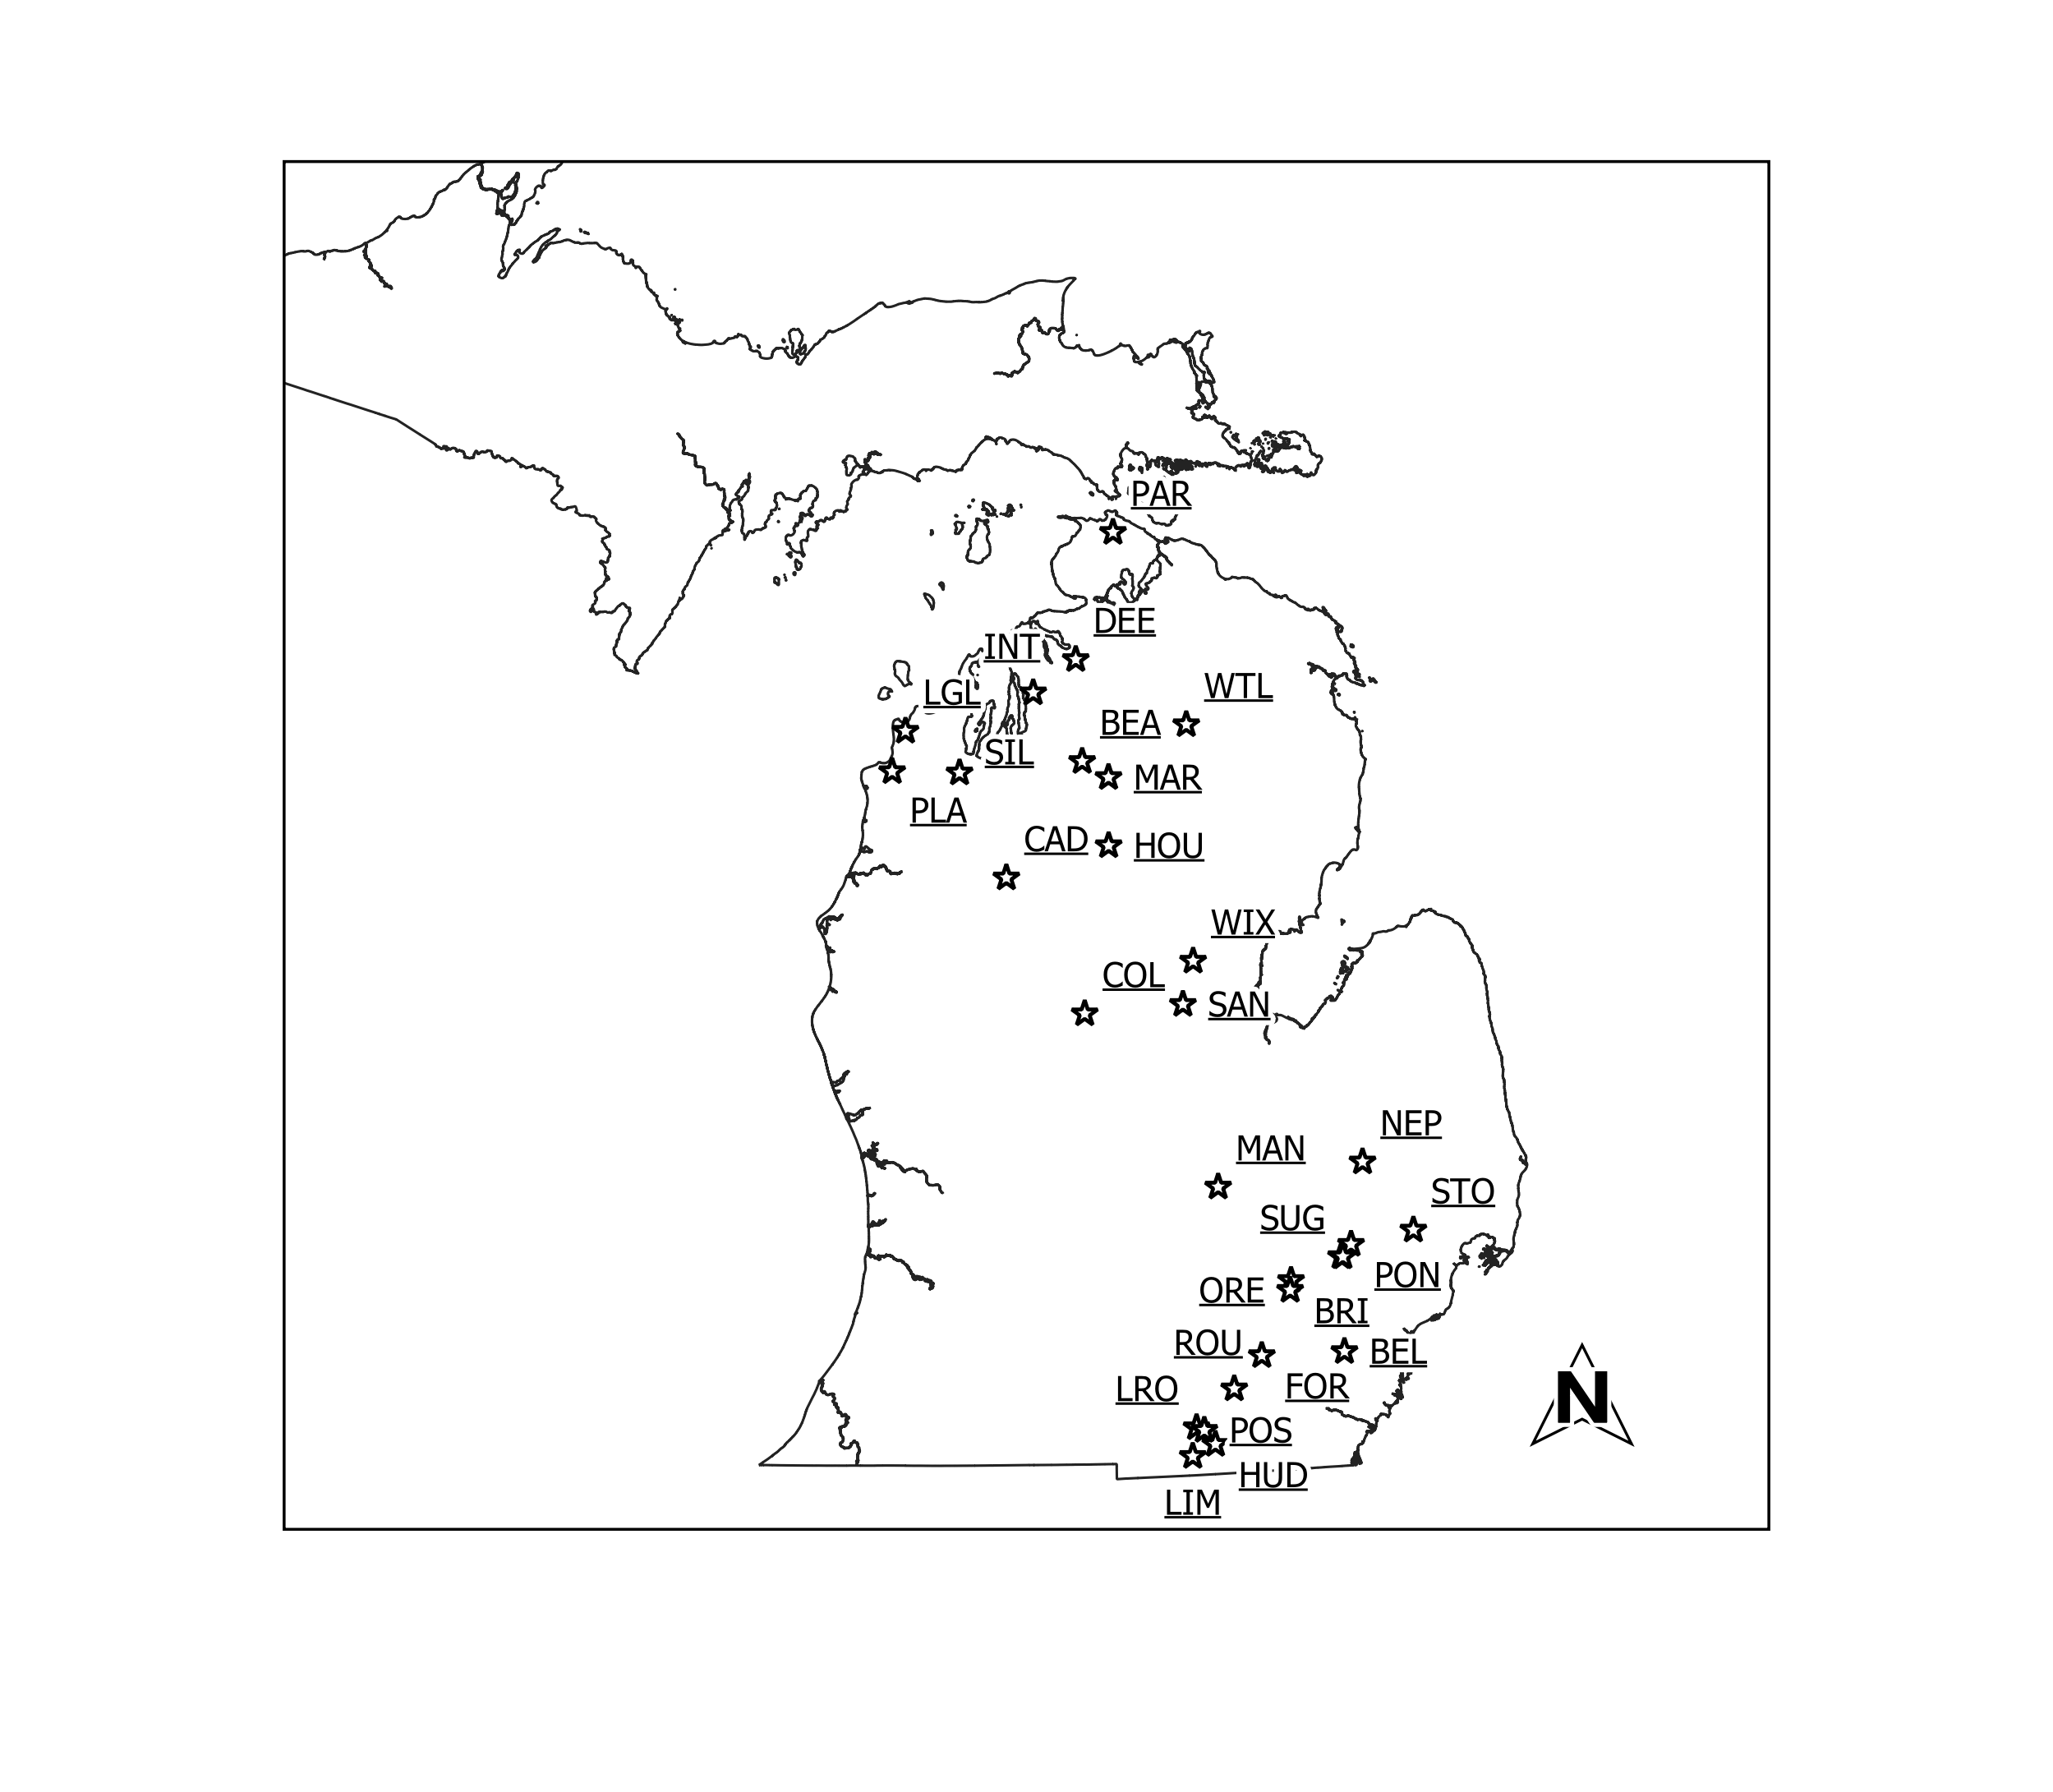
\includegraphics[width=\textwidth]{figures/Overview}
\label{overview}
\caption{Map of Sampled Lake Sites in Michigan}

\end{figure}

\begin{figure}[!ht]
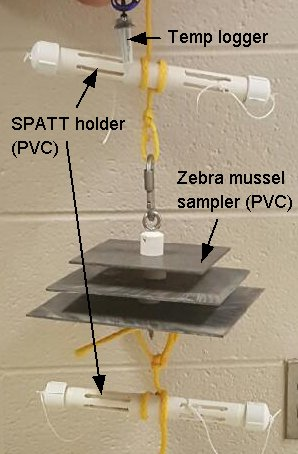
\includegraphics[width=\textwidth, angle =-90]{figures/samplers}
\caption{Picture of the constructed sampler installed at each lake}
\label{samplerr}
\end{figure}




\begin{figure}[!t]
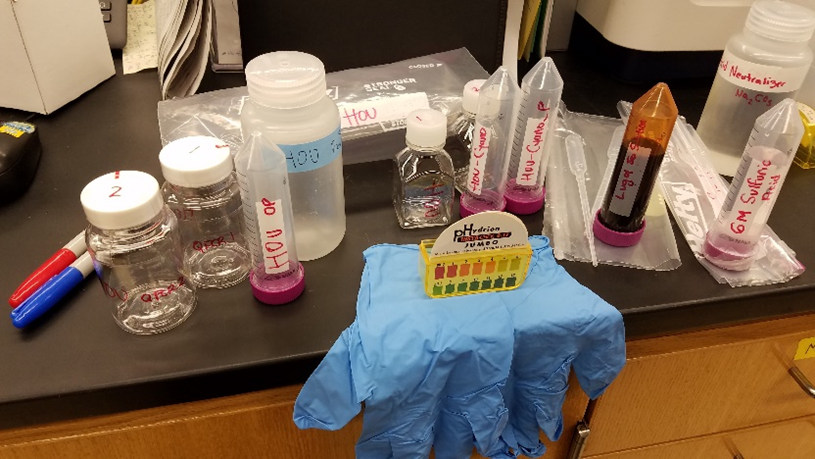
\includegraphics[width=\textwidth]{figures/samplekit}
\label{samplekit}
\end{figure}


\clearpage
\newpage

\section{Analysis}



\subsection{LC-MS/MS}

Water sample stored in 60mL PETG vials were freeze thawed for 3 cycles to lyse the cells.



A 3.5 ml aliquot of each sample above was transferred to glass vials suitable for the Thermo Scientific EQuan MAX (online sample concentrator).

Need to grab writeup from BRIAN was it filtered?????

These sample were transported to Wayne State University (WSU) and analyzed for 12 microcystin congeners, and nodularin.  The Westrick group at the WSU Lumigen Instrument Center (LIC) has developed a high-throughput LC-MS/MS analysis for microcystins in surface and drinking water analyses. The Westrick group’s LC-MS/MS platform includes a Thermo Scientific EQuan MAX (online sample concentrator) and ThermoFisher’s UltiMate 3000 (UHPLC) system and a TSQ Quantiva (MS/MS). The microcystin on-line concentration method is validated for 12 microcystins.

Their method is similar to EPA method 544 with the addition of 5 more congener analytes \cite{shoemaker_method_2015}. Figure \ref{spectra} shows a standard chromatogram of all 12 microcystins, nodularin, and the ethylated internal standard (C2D5 MC-LR) eluting between 2.2 – 5.2 minutes allowing for the total analyses time to be less than 12 minutes.  Minimum Detection limits (MDL) are 0.030  $\mu$g/L (or ppb) for microcystins.

\begin{figure}[h]
  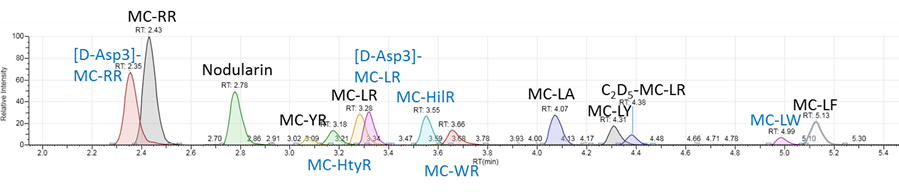
\includegraphics{LCMS_CONGENERS}
  \caption{Liquid chromotography-mass spectrometry chromatogram of the microcystin congeners}
  \label{spectra}
\end{figure}

\subsection{Nutrients}


Two 125-mL HPDE Nalgene bottles were used to collect acid-preserved water samples with 2mL of 3M \ch{H2SO4}, resulting to pH \textless 2. A 50 mL centrifuge tube is used to collect water sample without acid preservation for orthophosphate. One of the two nalgene bottle is allocated for ammonia-N and nitrate+nitrite-N by our lab at Oakland University and the other is for total phosphorus and total nitrogen run by Ben Southwell and his team at Lake Superior State University.  Samples were kept cool at 4 $^\circ$C during transport and stored at -20$^\circ$C. Upon receiving samples from field samplers samples are thawed if frozen and kept cool at 4$^\circ$C. All lake water samples are homogenized by inverting 8 times and aliquoted into 15-mL centrifuge vials and centrifuged at 3000rpm for 45 seconds. The supernatant was collected into a clean 3 mL vial and analyzed by AQ1 auto sampler. Ammonia-N is analyzed by an equivalent EPA method (USEPA Method 350.1), nitrate+nitrite-N analyzed by equivalent EPA method (USEPA Method 353.2), orthophosphate-P by equivalent EPA method (USEPA Method 365.1),total Kjeldahl nitrogen-N by equivalent EPA method (USEPA Method 351.2) and total phosphorus by equivalent EPA method (USEPA Method 365.1). All samples were analyzed within the appropriate time frame from time of sample.

\subsection{QPCR}

Phytoxigene CyanoDtec\texttrademark cyanobacteria and toxin test kit was preformed with Applied Biosystem StepOnePlus\texttrademark PCR. The kit provides two separate assay mix. Total cyanobacteria assay will quantify the 16srRNA gene copies found in the water sample. The toxin gene assay  were analyzed in parallel for each month of grab samples.  The PCR reaction mix contained 5 ul of template/sample extracts and 20 ul of rehydrated mastermix.  Each sample were run in singlicate due to limited amounts of reagent and budget. Positive standards for target genes  were run on each PCR analysis. CyanoNAS nucleic standards are removed from -20C and allowed to thaw prior to analysis.  Standards were run in duplicates.

Samples for QPCR were filtered either on site with portable Santino pump, or brought back to the lab for filtration within the day.
Each lake, 100mL or more of water sample was collected in a sterile IDEXX vessel then filtered through a 0.4$\mu$m pore size polycarbonate membrane  and stored at -20C until sampling route is back. Once filtered, they are immediately transferred into BioGX vials. BioGX vials are stored at -80C until analysis. BioGx vials contains 500 uL of lysis buffer, lysis beads and filtrate. For cell lysis, vials were vigorously shaken by bead beater for 2 minutes. After bead beaten, sample vials were centrifuged for 1 min. Supernatant was transferred to a microcentrifuge tube and centrifuged for 5 min, then transferred the final supernatant to another set of microcentrifuge tubes for PCR template.  Sample extracts are stored at 4C and analyzed within the day.



PCR heat cycles were programmed with initial denaturing step at 95$^\circ$C for 2 min, then a repeat of 95$^\circ$C for 15 seconds and 60$^\circ$C for 30 seconds reaching a total of 40 cycles. The appropriate gene targets filters were manually set to match the emission spectra of each probes. Each PCR run, standard curve is generated  from within the StepOnePlus software. CT threshold and baseline was manually assigned for each run by visually assessing each target run. The calculated gene copies are done automatically by the StepOnePlus software, expressed in gene copies/$\mu$L of lysate. The final reportable value is calculated by this equation:

\begin{center}
  $Genecopies/mL = (Genecopies/\mu L \: of \: lysate) \times (\frac{500\mu L \: of \: lysate}{\text{mL of Sample Volume}})$
\end{center}





\section{Watershed Characteristics}


Watershed delineation and calculation of land use was done using quantum geographic information system (QGIS) \cite{qgis_development_team_qgis_2009}.
Elevation data was downloaded in bulk by an FTP client as mosaic raster files for the state of Michigan downloaded from USGS (https://earthexplorer.usgs.gov/).
Elevation data  prepared by using $r.fill.dir$ function from GRASS which fills sinks or depressions \cite{grass_development_team_geographic_2017}. A flow accumulation raster map is generated from this command. The value of each cell designates the amount of flow based on drainage characteristics the elevation data. Visually viewing the histogram of the distribution of flow accumulation values, selecting the highest values displays will display the most probable areas the flow of water will be. This provided visual aid in selecting the pour point of each lake. A new shapefile was created and selected each lake's pour with the visual aid of stream flow lines. Using the $r.distance$ function from GRASS, i was able to snap each pour point to the proper place. Each lake's watershed was delineated using $r.drain$ to create a elevation model map derived from the flow accumulation raster file. The drainage raster file is then used as an input for function $r.water.outlet$ along with the coordinates of fixed pour point location, which gives the shape of each lake's watershed extent.

Land use data was downloaded from the 2006 National Land Cover Database \cite{development_completion_nodate}. The land use data were classified at anderson level-II, which has 20 different classification of land distinguishing different biomes and regions.  To simplify the land use data, the raster is reclassified into 8 anderson level-I categories using $r.recode$ tool from GRASS. The 8 anderson level-I classes are water, developed, barren, shrubs, forest, herbaceous and wetlands. Raster file was transformed into a vectorized shapefile. The shapefile was merged by union (or dissolved) by each lake's watershed, which resulted area of each land use class within each lake's watershed. This data was exported as a .csv file and prepared for statistical analysis.

Precipitation data were retrieved from the Global Historical Climatology Netowrk (GHCN) database from NOAA \cite{}. Daily precipitation data was downloaded from NOAA's FTP server (\url{ftp://ftp.ncdc.noaa.gov/pub/data/ghcn/daily/}).  The geolocation of each rain gauge station were imported into QGIS and mapped. The distribution of the rain gauges were not uniformally distributed. Thiessen/Voronoi polygons for each station were generated and overlayed on each watershed. The area of each thiessen/voronoi polygon's intersection with the corresponding catchmen is divided by the area of the lake's watershed to give a weighted value. The mean areal precipitation for each lake's watershed is calculated by taking each station's measurements and multiplying by the weighted value, then averaged together.  Ambient air temperature for each watershed is simply averaged together with their intersection of the lake's watershed. A multi-join was done in R using the \emph{dplyr} package for precipitation data with each sampled lake joined by lakes watershed \cite{wickham_dplyr:_2017}. Averaged 3, 5, 7, and 30 days lagged precipitation and ambient air temprature were calculated for our analysis.

\section{Statistical Modeling}

Each analytical measurement was compiled and organized by each sampling event. We have data sampled from Lake Superiour, Lake St. Clair and Lake Erie, however with my discussions with Dr. Szlag and Dr. Raffel, we decided to exclude them in our analysis.  Their unique geology and lake morphology does not fit our focus on inland lakes.
Data manipulation and analysis was done in Program R, a statistical computing language \cite{r_core_team_r:_2018}. The \emph{dplyr} package was used for data cleaning, compiling and preperation to have our dataset ready for statistical analysis \cite{wickham_dplyr:_2017}. Linear mixed models were used to analyze our data as this accounts for the variance of each of our lake site. The library package $lme4$ is used for our linear mixed modeling \cite{bates_fitting_2015}.

The requirements for building a linear model assumes the distribution of explanatory and response variables follow a normal distribution \cite{bates_fitting_2015}.
From our collected dataset, we assessed each variable's distribution and log-transformed to fit a normal distribution. To solve the problem of data values that are zero, we added the corresponding mininum detection limit first, then applied a log trasformation. See table \ref{variable} for a summary of which variable was transformed and the shorten variable name.

In our pursuit for finding important variables that potentially can explain our predictor variables, a best subsets regression analysis is used to find our features.  Measurements from each lake is a factor that may contribute as a random effect. This can be an issue where measurements from each lake is pseudoreplicated \cite{eisenhart_assumptions_1947}. Subset analysis is done on an averaged dataset based on each lake which works around this issue.
With the best variables from the regression subset, backward step-wise regression will be preformed to further refine the best fit model. Variables will be backwardly selected by F-test \cite{kenward_method_1987}. A linear mixed model will be used to verify our best models as it allows to account the variance of each sample site. Each non-nested models are rank by the lowest Bayesian Information Criterion (BIC) being our best model.
